The solution program plays sound effects and music, and is controlled by the eight buttons on the STK1000.
The LEDs are used to indicate which sound is playing.

When the program is started, the board is in idle mode, ready to react to button presses.
Pressing any of the buttons SW0-SW3 plays a piece of music, which loops until another sound is selected.
Pressing any of the buttons SW4-SW6 plays a sound effect, which is not looped.
Pressing SW7 stops all playback.

\subsection{Sound effects}

The sound effects are generatively composed by wrapping a generator signal in a configurable ADSR volume envelope.
TODO: talk about ADSR.
The available generator signals in the program are NOISE, SAWTOOTH and SQUARE.

TODO: talk about NISE, SAWTOOTH and SQUARE, with photos.
\begin{figure}[H]
	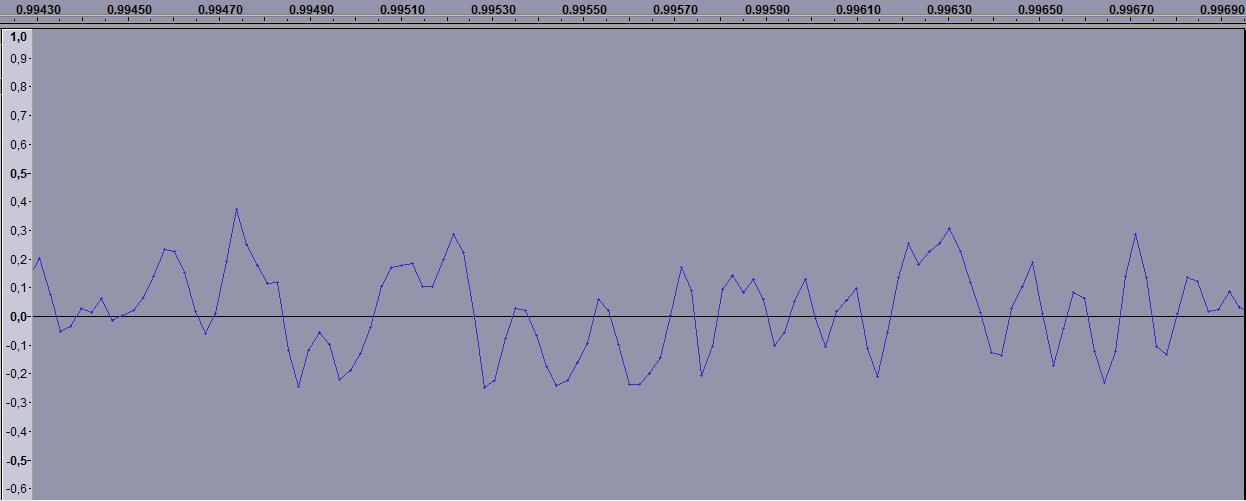
\includegraphics[width = \textwidth]{images/SW6zoom.png}
	\caption{}
	\label{img-sw6zoom}
\end{figure}

\begin{figure}[H]
	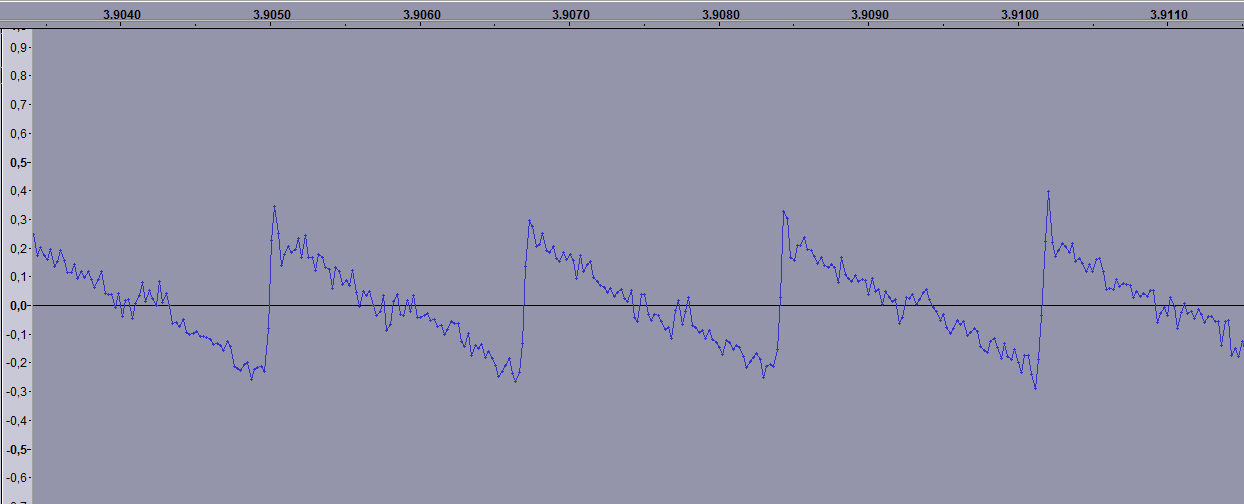
\includegraphics[width = \textwidth]{images/SW5zoom.png}
	\caption{}
	\label{img-sw5zoom}
\end{figure}

\begin{figure}[H]
	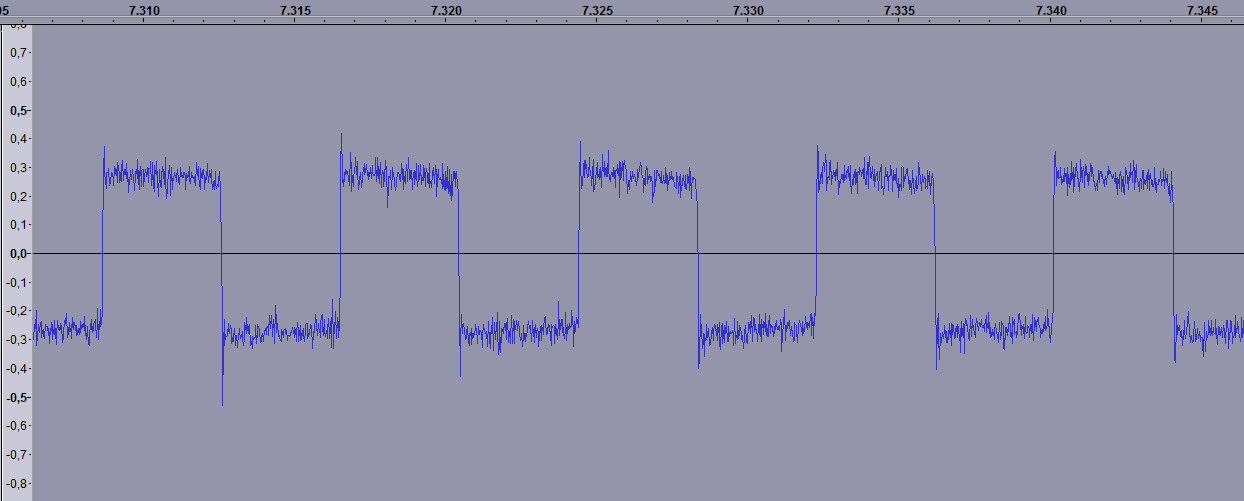
\includegraphics[width = \textwidth]{images/SW4zoom.png}
	\caption{}
	\label{img-sw4zoom}
\end{figure}

\subsubsection{Explosion}

'Explosion' is a NOISE-based sound effect with the following ADSR envelope:
Attack: 0 ms
Decay:  1000 ms
Sustain: 0\%
Release: 0 ms
The effect is held for 0 ms.

Total length: 0 ms + 1000 ms + 0 ms + 0 ms = 1000 ms
'Explosion' can be triggered by pressing SW6.
TODO ref image

\begin{figure}[H]
	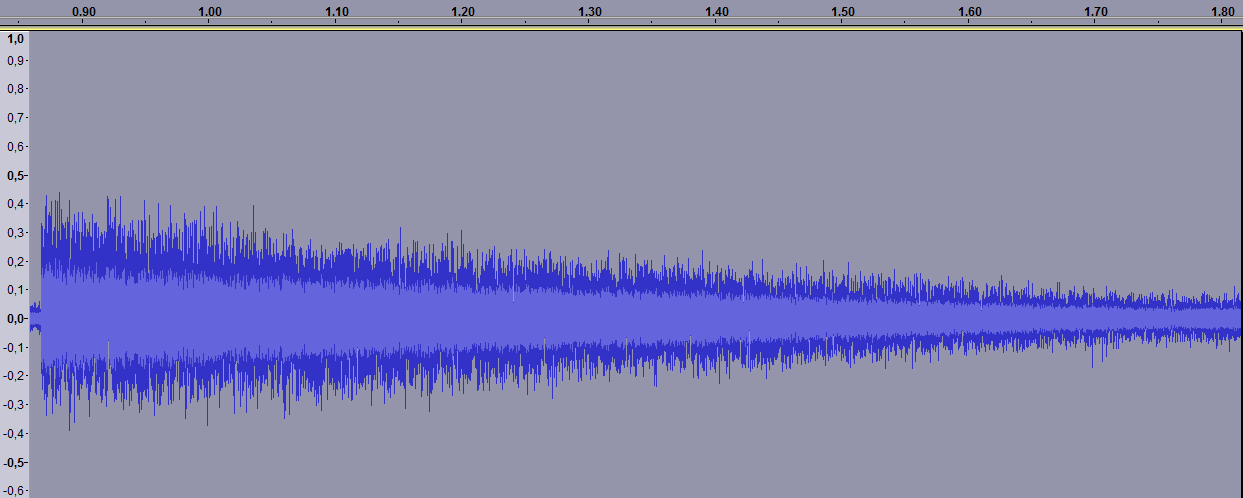
\includegraphics[width = \textwidth]{images/SW6.png}
	\caption{}
	\label{img-protracker}
\end{figure}


\subsubsection{Air horn}
'Air horn' is a SAWTOOTH-based sound effect with the following ADSR envelope:
Attack: 100 ms
Decay:  100 ms
Sustain: 70\%
Release: 500 ms
The effect is held for 0 ms.

Total length: 100 ms + 100 ms + 500 ms + 0 ms = 700 ms
'Air horn' can be triggered by pressing SW5.
TODO ref image

\begin{figure}[H]
	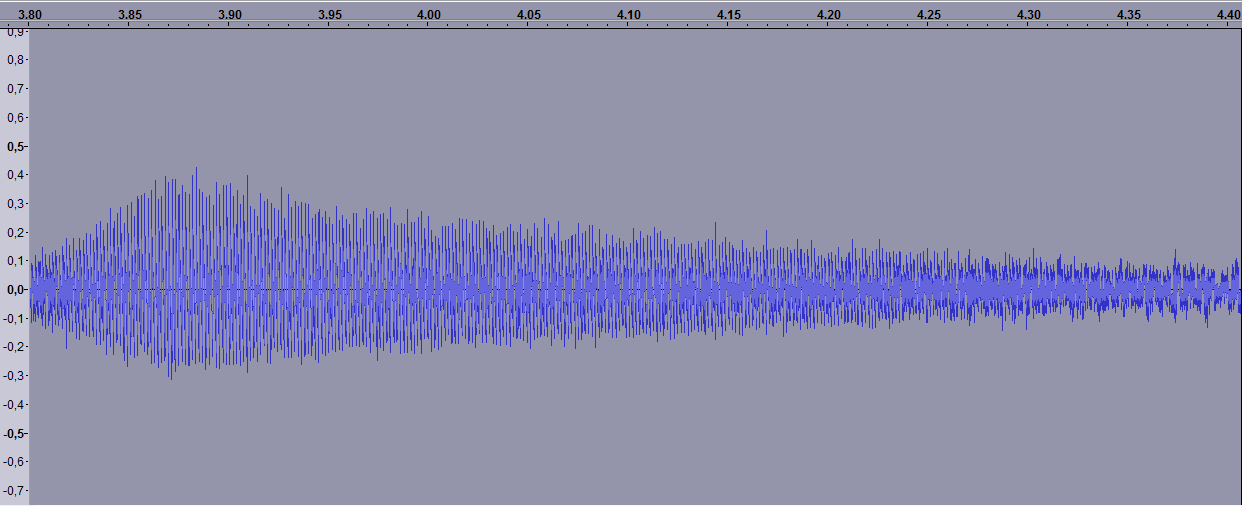
\includegraphics[width = \textwidth]{images/SW5.png}
	\caption{}
	\label{img-protracker}
\end{figure}

\subsubsection{Teleport}
'Teleport' is a SQUARE-based sound effect with the following ADSR envelope:
Attack: 500 ms
Decay:  1250 ms
Sustain: 20\%
Release: 250 ms
The effect is held for 0 ms.

Length: 500 ms + 1250 ms + 250 ms + 0 ms = 2000 ms
'Teleport' can be triggered by pressing SW4.
TODO ref image

\begin{figure}[H]
	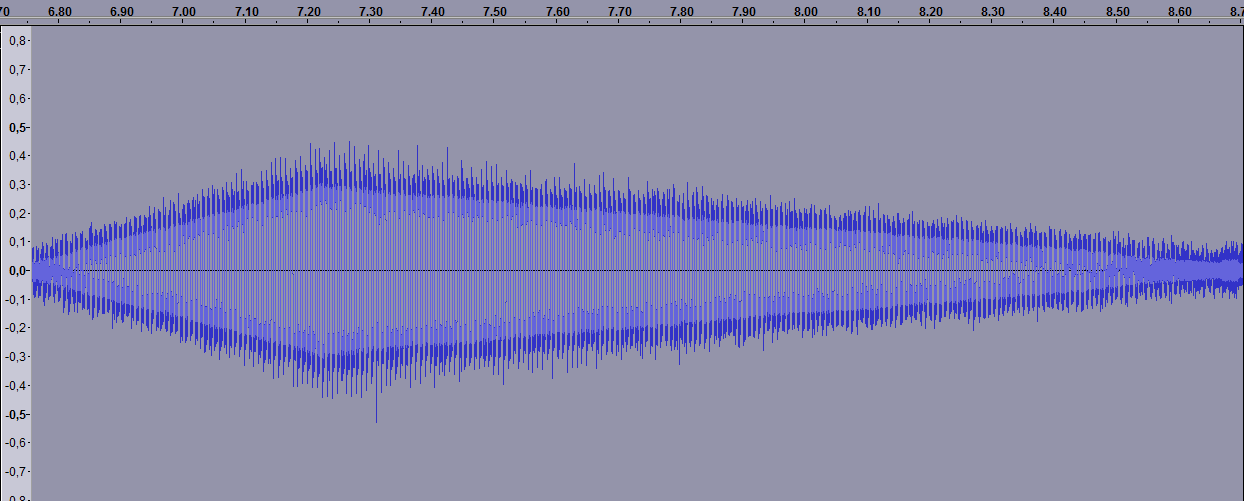
\includegraphics[width = \textwidth]{images/SW4.png}
	\caption{}
	\label{img-protracker}
\end{figure}


\subsection{Music}

The music pieces in the solution program are played by the MOD player.

\subsubsection{Tuulenvire by Dizzy/CNCD}
Tuulenvire is a 2:09 long 808KB composition in the ambient genre, featuring piano and accordion, amongst other instruments.
This composition was chosen to demonstrate how careful composing can render realistic compositions with a relatively small memory footprint.
It uses 25 different PCM-coded sounds.
Tuulenvire can be triggered by pressing SW3.

\subsubsection{Boesendorfer P. S. S. by Romeo Knight}
Boesendorfer P. S. S. is a 3:22 long 211KB solo piano composition, chosen to illustrate the possibilities enabled by a hybrid generative/recorded approach.
It uses 9 different PCM-coded sounds.
Boesendorfer P. S. S. can be triggered by pressing SW2.

\subsubsection{Drop The Panic by H0ffmann}
Drop The Panic is a 4:05 long 702KB ``glitch-hop'' composition.
It was chosen to show how MOD files can support embedded vocals.
It uses 31 different PCM-coded sounds.
The composition was tweaked by adding some extra inaudible notes in the beginning of the song to decrease critical cache misses by the MOD player during playback on the STK1000.
Drop The Panic can be triggered by pressing SW1.

\subsubsection{Bacongrytor by Maktone}
Bacongrytor is a 15Kb endless loop chiptune-style composition, chosen to demonstrate the compactness of the MOD format, and therefore its aptfulness for use on microcontrollers.
It uses 7 different PCM-coded sounds.
Bacongrytor can be triggered by pressing SW0.
